\chapter{Motivación del trabajo}
\label{chap:intro}

\drop{E}{l} \textbf{senderismo} se ha convertido en una de las prácticas deportivas preferidas por los españoles. Podemos darnos cuenta de ello si echamos un vistazo a los datos del año 2017 \cite{FED}, con más de $112$.$000$ personas federadas según la \ac{FEDME}. De entre los federados, según un estudio de la \ac{FEDME} \cite{2} un $96,7$ \% de los encuestados practican senderismo y un $86,1$ \% practican montañismo. Si tenemos en cuenta también las licencias autonómicas, el número de afiliados sube hasta más de $200$.$000$. Según datos del \ac{CSD} \cite{CSD}, se puede observar que el senderismo ocupa el quinto lugar en la lista de deportes con más federados.

La relación entre el hombre y la montaña \cite{11} es tan antigua como la propia humanidad, ya que gracias a la montaña el hombre ha podido satisfacer sus necesidades, las cuales han ido cambiando a lo largo del tiempo. De ser un simple lazo natural en los inicios de la humanidad, a ser hoy en día un entorno social dónde las personas pueden compartir sus inquietudes. Las prácticas sociales más desarrolladas en la montaña son aquellas que tienen que ver con la expedición, bien sea en solitario o en grupos de expedición.

Los grupos de expedición son cada vez más numerosos, encontrándose en ellos senderistas con distinto nivel de experiencia en la montaña. Muchos senderistas se lanzan a la aventura, sin experiencia y sin conocer las dificultades que presentará el terreno, por lo que la existencia de un guía en los grupos de expedición es clave. En estos grupos hay personas de distinto nivel y forma física, por lo que hacer una ruta apta para todo el mundo (tanto en recorrido, como en velocidad de marcha) puede llegar a ser una tarea complicada para el guía. Además, el guía es el responsable de la seguridad de los senderistas y en grupos numerosos es más difícil tener controlados todos los riesgos sin el uso de mecansimos de monitorización y control. En el año 2016, un $0,16$ \% de los federados tuvo que ser rescatado \cite{4}. 

Conforme los senderistas van completando rutas, empiezan a buscar otras de más duración, que transcurran por lugares más difíciles y en medios más hostiles (nieve, agua, zonas rocosas), rutas en las que existen menos señales que identifiquen el camino, etc. En definitiva, rutas en las que la seguridad es un factor clave. 

La expedición en la montaña puede resultar peligrosa. Precisamente, la peligrosidad es un factor que los humanos encuentran motivante y no es sorprendente que se busquen actividades con este factor de peligrosidad. Las actividades peligrosas hacen que las personas puedan volverse adictas a la adrenalina \cite{15}. La adrenalina es un neurotransmisor que provoca excitación, por lo que el cerebro puede desensibilizarse a esta hormona una vez que ha sido expuesto a la misma y la única forma de obtener una sensación igual es aumentar la peligrosidad de la actividad. Según el estudio \cite{12}, los individuos con mayor experiencia son más propensos a esta desensibilización, ya que buscan sentimientos relacionados con la euforia, el desafío personal y la toma de decisiones, mientras que los individuos con menor experiencia buscan la participación en actividades sociales y el sentimiento de evasión.

Además hay otros factores que están realacionados directamente con la peligrosidad, como puede ser la dispersión del grupo de expedición. Un grupo muy disperso es difícil de controlar y por tanto, es más propenso a sufrir accidentes. La rápida actuación ante un accidente, como puede ser la caída de un miembro del grupo, es clave para minimizar el impacto de la caída, por lo que el grado de dispersión es una cuestión a tener controlada. Cuanto menor sea este grado de dispersión, más rápida será la actuación ante un accidente. Los factores meteorológicos como la lluvia y la iluminación del ambiente también son claves en el aumento de la peligrosidad.

A grandes altitudes (por encima de los 2500 metros) \cite{13}, el riesgo y el peligro aumenta en los senderistas. El principal peligro es el llamado <<mal de altura>>. Con el crecimiento de la expedición en la montaña, y la participación de gente inexperta, los accidentes en la misma aumentan, ya sea por una baja preparación o por comportamientos inadecuados. Los guías de expedición, intentan minimizar los accidentes, priorizando la seguridad. Por esto, es crucial que los guías tengan mecanismos que les faciliten esta tarea.

Con el auge del senderismo se han empezado a comercializar bastantes dispositivos cuyo objetivo es la mejora de la seguridad para los senderistas, los cuales poseen \acs{GPS}, sensor de frecuencia cardiaca, herramientas para medir altitud y otros datos relevantes. Cabe destacar que son dispositivos de alto coste, con la mayoría por encima de los 300-400 euros. También, han nacido aplicaciones de tipo social que buscan el seguimiento de las rutas individuales y la competitividad entre los usuarios en ciertos tramos de esas rutas.

El factor común de estas aplicaciones y dispositivos es la individualidad. Con estas aplicaciones no se resuelve la problemática del control de un grupo, para maximizar la seguridad de sus miembros. Sigue siendo difícil la correcta comunicación de los guías con los miembros de su grupo, que con un simple golpe de vista sepa dónde se encuentran los senderistas para evitar que los mismos se pierdan por el camino, además de llevar un control sobre el estado de salud de cada uno de los miembros del grupo.

Los dispositivos usados en expediciones en la montaña deben tener algunos requisitos especiales \cite{14}, como son la capacidad de trabajar en tiempo real. La información que proporcionan estos dispositivos (por ejemplo parámetros de localización, altitud, salud física, etc.) debe estar disponible de forma casi inmediata. Además, no es viable portar un dispositivo de grandes dimensiones, por comodidad del senderista al llevarlo encima (deben ser dispositivos con poco peso y de dimensiones reducidas). Se suelen utilizar, por tanto, dispositivos pequeños y de bajo poder de cómputo, por lo que la eficiencia en la programación de estos dispositivos es clave. 

En este contexto nace este proyecto, como una herramienta para monitorizar los eventos que se puedan producir en un grupo de expedición y para ayudar a los guías a tomar decisiones para maximizar la seguridad de los integrantes durante la expedición. 

Para maximizar la eficiencia se tendrán en cuenta diseños de \textit{hardware} empotrado sobre un microcontrolador. De esta forma, el diseño se centrará en resolver la problemática planteada por lo que la productividad será mayor que usando un sistema de propósito general. Además, con arquitecturas de \textit{hardware} embebido, se resuelve fácilmente la cuestión de la computación en tiempo real.

De acuerdo a esta problemática se pretende realizar, por tanto, un dispositivo \textit{hardware} equipado con varios sensores, que permita recoger la información necesaria del entorno. Este dispositivo consistirá en un microcontrolador Arduino \cite{9} equipado con sensores adecuados para la monitorización del grupo de expadición, que tomará la información recibida de los mismos \cite{8} y la enviará a un dispositivo móvil conectado con el microcontrolador. 

Se desarrollará también una aplicación móvil \cite{10} que tomará todos los datos provenientes del microcontrolador y realizará un procesamiento inteligente y en tiempo real de los mismos, para detectar posibles situaciones de riesgo como pueden ser caídas, una gran dispersión de los miembros del grupo o condiciones climatológicas adversas entre otras. Esta información será presentada a los miembros de la expedición a través de una interfaz. 

Por último, se va a desarrollar una plataforma web, que servirá para mostrar un histórico de todas las expediciones que el senderista ha realizad. Se mostrarán las estadísticas de la expedición de una forma amigable. Esta plataforma web también podrá ser usada por la familia o amigos de los senderistas para visualizar en tiempo real los datos del senderista en la expedición. 

Con esta propuesta se pretende cubrir el vacío que existe en dispositivos y aplicaciones para el control de grupos de senderismo ya que se tendrán en cuenta los datos recibidos de todas las personas para hacer un procesamiento conjunto y mostrar la información relevante. 

El proyecto servirá a los guías de estos grupos que verán en todo momento dónde se encuentran los senderistas y su estado de salud, entre otra información, y les servirá para tomar decisiones de una forma más fácil sobre si continuar la marcha, bajar el ritmo de la misma, hacer una parada para una reagrupación, etc. Con este proyecto se mejorará la seguridad de los senderistas, ya que ante la identificación de caídas \cite{7} o empeoramiento del estado de salud se enviará un mensaje al guía para que actúe en consecuencia. 

\section{Trabajos previos}

\subsection{Aplicaciones existentes para rutas de expedición}

Es notorio destacar que apenas existe alguna aplicación con una funcionalidad parecida a la que se expone en el presente proyecto. La mayoría de aplicaciones para dispositivos móviles que se encuentran tienen que ver con la gestión de rutas en la montaña y la predicción de la climatología. Ninguna de ellas se enfrenta al problema del control de un grupo de senderismo ya que están enfocadas de forma individual. Por tanto, existe un vacío en lo referente a aplicaciones que permitan mejorar la seguridad de un grupo de expedición.

\paragraph{AllTrails}

\textit{AllTrails} es una aplicación móvil para iOS y Android que permite la búsqueda de nuevas rutas de expedición además de conocer a otros senderistas. \textit{AllTrails} permite la búsqueda de rutas cercanas, a partir de la localización \ac{GPS} actual. Esta aplicación proporciona algunos consejos acerca de obstáculos en el camino e información sobre lugares importantes cercanos a la ruta que se está realizando. La descarga de la aplicación es gratuita, tanto en iOS como en Android pero para el acceso a contenido más avanzado, como la descarga de mapas \textit{offline}, es necesario pagar una suscripción.

\paragraph{GPX Viewer}

\textit{GPX Viewer} es una aplicación móvil y de escritorio que permite evitar problemas de orientación. Esta aplicación permite cargar rutas previamente descargadas de internet en varios formatos y visualizarlas después sobre \textit{Google Maps}. Con esta aplicación es posible también guardar tus movimientos para crear la ruta por la que transcurres sobre un mapa. Esta ruta se podrá almacenar en el dispositivo para visualizarla posteriormente o para volver a reproducirla en cualquier otro momento. 


\begin{figure}[!htb]
   \begin{minipage}{0.48\textwidth}
     \centering
     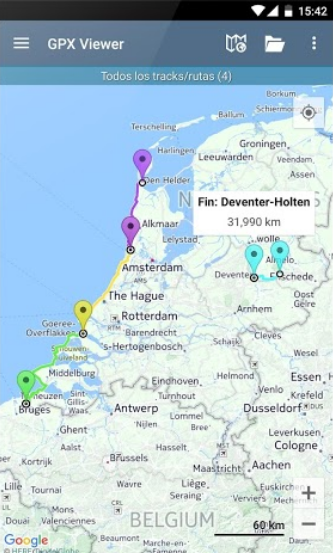
\includegraphics[width=.5\textwidth]{gpxviewer.png}
	\caption{Aplicación móvil \textit{GPX Viewer}. \protect\footnotemark}
	\label{fig:gpxviewer}
   \end{minipage}\hfill
   \begin{minipage}{0.48\textwidth}
     \centering
     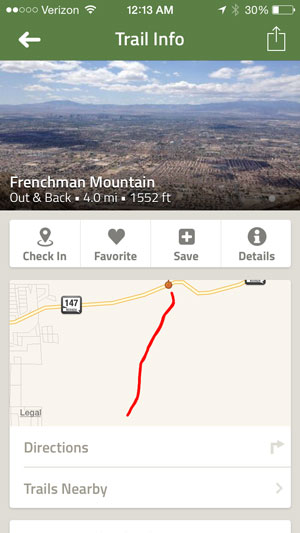
\includegraphics[width=.5\textwidth]{alltrails.jpg}
	 \caption{Aplicación móvil \textit{AllTrails}. \protect\footnotemark}
	 \label{fig:alltrails}
   \end{minipage}
\end{figure}

\footnotetext{Imagenes originales extraídas de \url{https://play.google.com/store/apps/details?id=com.vecturagames.android.app.gpxviewer&hl=es} y de \url{https://bearfoottheory.com/find-local-hiking-trail}}

\paragraph{Primeros Auxilios - Cruz Roja}

Se trata de una aplicación móvil desarrollada por la Cruz Roja con el objetivo de enfrentarse a las emergencias cotidianas. Esta aplicación proporciona consejos, información interactiva y mediante vídeos para guíar al usuario en los primeros auxilios del día a día. Es una aplicación útil para saber como reaccionar ante crisis de asma, sangrados, lipotimias y otras situaciones que pueden ocurrir en la montaña. además, es una aplicación que funciona sin cobertura y tiene una lista con contactos de urgencia para llamar a servicios de emergencias de una forma rápida y sencilla.

\paragraph{Alpify}

Esta aplicación móvil multiplataforma (iOS y Android) desarrollada por \texttt{Safe365}\footnote{\url{https://safe365.com/es/}} se centra en el auxilio rápido de un accidentado en la montaña o practicando cualquier otro deporte como puede ser el ciclismo. Es una aplicación necesaria en el caso de accidentes o cambios bruscos de climatología que posee un gran botón rojo central que en el caso de ser pulsado envía la localización exacta en la que te encuentras y realiza una llamada al servicio de emergencias. En el caso de no haber cobertura, se envía un mensaje de texto por \ac{SMS}. Se le puede facilitar a la aplicación un teléfono de contacto de algun amigo o familiar. La aplicación comunicará este número de teléfono automáticamente a los servicios de emergencias para que éstos puedan ponerse en contacto con los allegados del accidentado. En el caso en el que el accidente haya sido un desmayo y al senderista no le haya dado tiempo a pulsar el botón, una vez que se haya producido la denuncia de desaparición, \texttt{Safe365} tendrá todos los datos de la ruta, algo que puede ser de utilidad para los servicios de rescate.

\begin{figure}[!htb]
\begin{minipage}{0.48\textwidth}
\centering
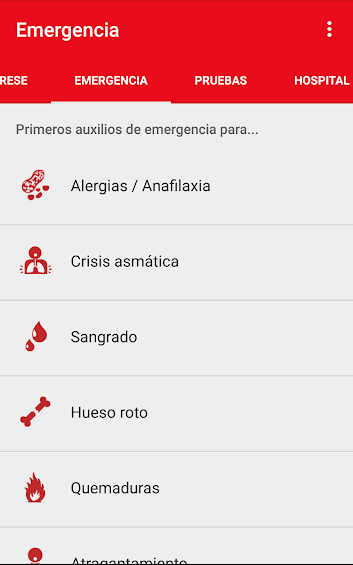
\includegraphics[width=0.5\textwidth]{primeros_auxilios.png}
\caption{Aplicación móvil Primeros Auxilios. \protect\footnotemark}
\label{fig:primeros_auxilios}
\end{minipage}\hfill
\begin{minipage}{0.48\textwidth}
\centering
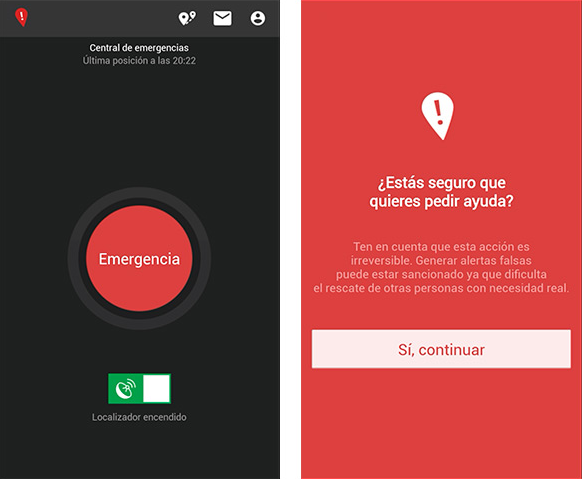
\includegraphics[width=1\textwidth]{alpify.png}
\caption{Aplicación móvil \textit{Alpify}.}
\label{fig:alpify}
\end{minipage}
\end{figure}

\footnotetext{Imagen original extraída de \url{https://play.google.com/store/apps/details?id=com.cube.arc.fa&hl=es_419}}

\subsection{Dispositivos existentes para rutas de expedición}

Al igual que se ha comentado en el punto anterior con las aplicaciones existentes en el mercado para rutas de expedición, no existen dispositivos con una funcionalidad igual o muy parecida a la del dispositivo que se expone en el presente proyecto. La mayoría de dispositivos en el mercado están centrados en maximizar la seguridad individual, para responder de forma rápida ante accidentes. También se pueden encontrar muchos dispositivos de monitorización individual, que se encargan de tomar información sobre el portador del mismo (información de localización, de pulso cardíaco, de altitud y de carácter social, entre otras). 

\paragraph{\acs{ARVA}}

Un \ac{ARVA} (véase Figura \ref{fig:arva}), o dispositivo de búsqueda de víctimas de avalanchas, es un aparato que emite de forma continua una señal emisora muy potente que se puede detectar incluso bajo una gran capa de nieve, al quedar el montañista sepultado por un alud en la montaña. Los equipos de rescate y otros compañeros de expedición llevan otros dispositivos \ac{ARVA}, que si se ponen en modo de recepción, se usan para recoger la señal del \ac{ARVA} del montañista sepultado y localizar con una gran exactitud al mismo. 

Cuando un montañista sale de expedición con un \ac{ARVA} entre su equipo, este tiene que ir siempre con el montañista y nunca en la mochila u otro objeto que no sea él mismo. Esto es debido a que ante avalanchas de nieve, es posible que la mochila se pierda y se separe del montañista por lo que la señal del \ac{ARVA} indicaría la localización de la mochila y no del montañista. También es importante que el \ac{ARVA} vaya debajo de nuestra ropa para que en caso de avalancha no entre en contacto directo con la humedad de la nieve y las baterías duren más. Hay que intentar colocarlo en zonas blandas del cuerpo para que en caso de caída, no nos produzca fisuras en huesos. Además, el \ac{ARVA} debe estar en modo de emisión y el modo recepción tiene que estar restringido a búsqueda de compañeros. 

Hoy en día las mochilas más técnicas traen incorporado un \ac{ARVA}. Esto le resulta muy cómodo al montañista ya que no necesita portar ningún otro dispositivo mas allá de su chaqueta. 

Inicialmente, los \ac{ARVA} transmitían a una frecuencia de $2275$kHz, pero en el año 1986 se estableció un estándar para que todos estos dispositivos emitiesen a una frecuencia de 457kHz. Todos los dispositivos \ac{ARVA}, sea cual sea su marca, son comptabiles entre si, consiguiendo así que cualquier portador de un dispositivo \ac{ARVA} sea capaz de localizar otro dispositivo cualquiera y asegurando que si un montañista se queda atrapado con su \ac{ARVA} emitiendo, podrá ser encontrado por cualquier otro \ac{ARVA} de cualquier marca. 

\begin{figure}[!h]
\begin{center}
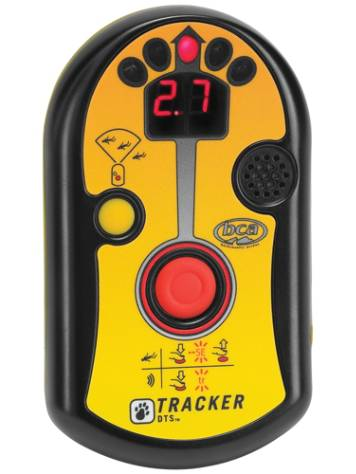
\includegraphics[width=0.25\textwidth]{arva.jpg}
\caption{Dispositivo \ac{ARVA} para la búsqueda de montañistas en avalanchas. \protect\footnotemark}
\label{fig:arva}
\end{center}
\end{figure}

\footnotetext{Imagen original extraída de \url{https://images.blue-tomato.com/is/image/bluetomato/301529492_front.jpg-vKXjlekI60xiNRwUj6n0Y-rZL04/Tracker+Dts+ARVA.jpg?\$b1\$}}

Según \cite{41} de 105 personas enterradas y rescatadas por aludes, antes de que transcurriesen 15 minutos desde que fueron sepultadas, 98 fueron encontradas con vida y 7 personas fueron encontradas muertas. Esto se corresponde con que un 93\% de las personas fueron encontradas con vida entre los minutos 0 y 15 después de su accidente. Cabe destacar que entre los minutos 15 y 45, el porcentaje de encontrar a una persona con vida se reduce hasta un 26\%, por lo que los primeros minutos después de una avalancha son cruciales. Por eso es importante portar un \ac{ARVA} en tu equipo de expedición, ya que es un dispositivo que precisamente intenta minimizar el tiempo de búsqueda de desaparecidos. 

Además es importante que tus compañeros de expedición porten también un \ac{ARVA} y sepan usarlo ante situaciones de emergencia, ya que según este estudio un 71\% de las víctimas de aludes socorridas por compañeros de expedición sobreviven, frente a un 13\% de montañistas recogidos con vida por los cuerpos de socorro. Esto se debe principalmente a la criticidad de encontrar al montañista sepultado en los primeros 15 minutos, después de haber ocurrido el alud. 

Existen dos tipos de dispositivos \ac{ARVA}, los dispositivos analógicos y los digitales. Cuando un \ac{ARVA} analógico se encuentra en un estado de recepción e intercepta una señal de otro \ac{ARVA} que se encuentra en estado de emisión, se encarga de amplificarla y emitir un sonido sonoro ``\textit{bip}'' que es más intenso cuanto más cerca se encuentre de la fuente de emisión de señales. Los dispositivos digitales convierten las señales procedentes del \ac{ARVA} en estado de emisión a indicadores visuales (mediante un microprocesador interno). Estos indicadores pueden ser flechas que muestran la dirección y aumentan la intensidad de sus colores conforme nos acercamos a la fuente de la señal. Los indicadores pueden ser también numéricos, que nos indican la distancia (no necesariamente medida en metros) a la fuente de emisión. Cuanto más cerca estemos, más pequeños seran estos valores numéricos. 

\paragraph{Sonda}

Una sonda consiste en una vara larga (en torno a unos dos metros y medio) y plegable, cuyo principal objetivo es determinar a qué profundidad se encuentra enterrada la víctima. Es una buen complemento a un \ac{ARVA}, ya que éstos nos dan una precisión bastante exacata pero con la sonda, la precisión es la máxima posible. Una vez que se ha llegado al punto en el que el \ac{ARVA} da la máxima señal, hay que proceder al sondeo, realizando círculos concéntricos y con una señaración entre ellos de unos 25 centímetros. Cuando tenemos localizada a la víctima con una gran precisión, habrá que dejar clavada la sonda en ese lugar perpendicular a la pendiente. Hay que evitar pisar en la zona para no destruir las posibles bolsas de aire que se hayan creado y puedan ayudar a respirar al montañista sepultado.

\begin{figure}[!h]
\begin{center}
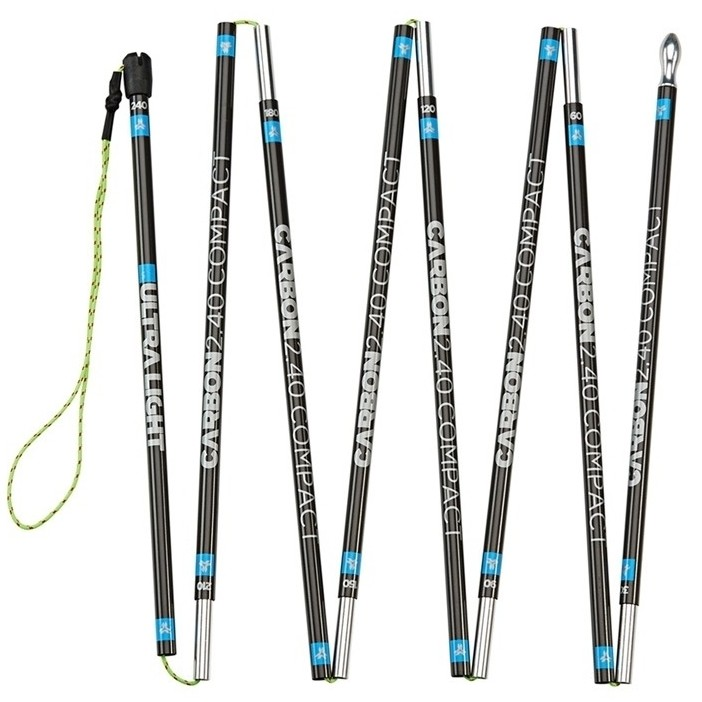
\includegraphics[width=0.30\textwidth]{sonda.jpg}
\caption{Sonda de fibra de carbono. \protect\footnotemark}
\label{fig:sonda}
\end{center}
\end{figure}

\footnotetext{Imagen original extraída de \url{https://static.forumsport.com/img/productos/1000x1000/ARVA\%20VARIOS\%20MONTA\%C3\%91A\%20SONDA\%20CARBON\%202.40\%20COMPACT-430360.jpg}}

\paragraph{\acs{PLB}}

Las \ac{PLB} o balizas personales de localización son unos dispositivos creados para el rescate en la montaña y en aguas abiertas. Estos dispositivos envían una señal de emergencia cuando el afectado se encuentra en una situación de peligro de muerte o situación \ac{MOB}. Estas balizas transmiten la posición con una gran precisión a servicios de búsqueda y salvamento a través de los satélites \ac{LEOSAR} y \ac{GEOSAR}. Los servicios de salvamento son internacionales y se fundaron por cuatro países (Estados Unidos, Canadá, Francia y Rusia), extendiéndose en la actualidad hasta 43 países. Cuando reciben una alerta, notifican a servicios de búsqueda locales, que procederán al rescate del afectado.

Un inconveniente de las \ac{PLB} es que una vez activada la alerta no se puede cancelar, por lo que si se emite una alerta de forma accidental no existe una manera para comunicar el falso positivo. Además, cuando se compra una \ac{PLB}, hay que registrarla (de forma gratuita) ante una autoridad nacional ya que si no se hace, la baliza es totalmente inútil. En este registro, se indican datos personales como el nombre, la dirección, un número de contacto en caso de emergencia, etc. además de datos médicos, para minimizar el tiempo de respuesta de los equipos médicos en un rescate. Estos datos se deben actualizar cada dos años y si cambia el dueño de una \ac{PLB}, se debe reportar para almacenar los datos del dueño actual. 

\begin{figure}[!h]
\begin{center}
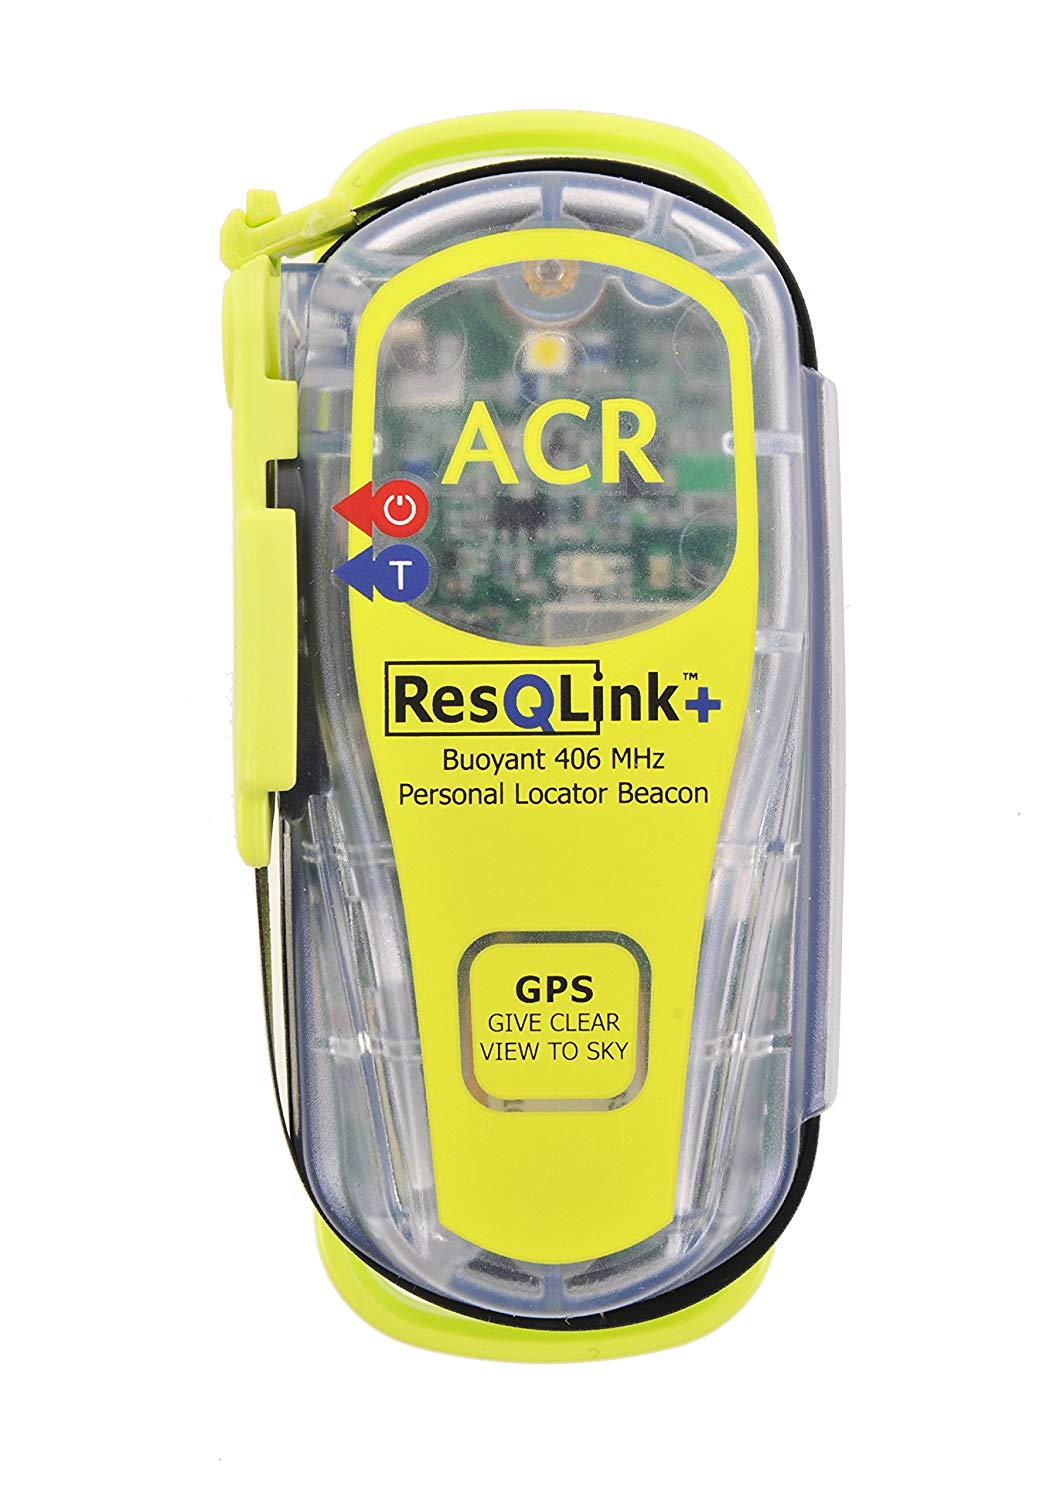
\includegraphics[width=0.30\textwidth]{plb.jpg}
\caption{Baliza \ac{PLB} para la localización y rescate de accidentados. \protect\footnotemark}
\label{fig:plb}
\end{center}
\end{figure}

\footnotetext{Imagen original extraída de \url{https://images-na.ssl-images-amazon.com/images/I/81fx0wksbtL._SL1500_.jpg}}

Las \ac{PLB} tienen baterías de gran duración (pueden durar hasta cinco años) que permanecen en un estado inactivo hasta que se activa la \ac{PLB}. Estas baterías son capaces de funcionar en condiciones extremas (pueden transmitir señales a temperaturas inferiores a los -20ºC). Sin embargo, los cambios de batería suelen ser caros y requieren enviar el dispositivo completo para realizar este cambio de batería. 

\paragraph{\textit{Satellite Messengers}}

Los dispositivos de notificación por satélite o \acx{SEND} \cite{42} se usan para realizar una comunicación por mensajes de texto en caso de emergencia, con algún familiar o con los equipos de rescate. Al contrario que las \ac{PLB}, los mensajes enviados con los dispositivos de notificación por satélite no son gratuitos. Estos dispositivos no usan la misma red de satélites que las \ac{PLB} y normalmente no tienen cobertura en ciertas zonas de Alaska y en la Antártida, por lo que antes de viajar a algún área remota es necesario comprobar la cobertura en ese lugar.

Los equipos de rescate prefieren el uso de este tipo de dispositivos ya que se puede cancelar una falsa alarma y evita costes innecesarios derivados de un falso positivo. Se han desarrollado incluso aplicaciones móviles (como \texttt{Earthmate}\footnote{\url{https://buy.garmin.com/es-ES/ES/p/577212}}) que permiten conectar el dispositivo de notificación por satélite con el teléfono móvil para facilitar el intercambio de mensajes.

\begin{figure}[!h]
\begin{center}
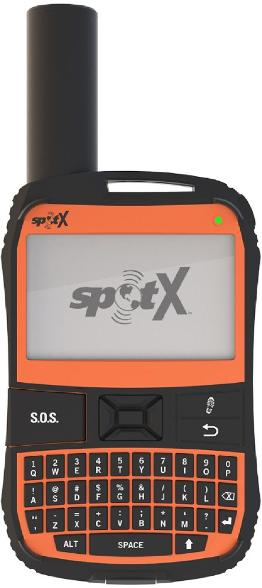
\includegraphics[width=0.20\textwidth]{messenger.jpeg}
\caption{Dispositivo de notificación por satélite. \protect\footnotemark}
\label{fig:messenger}
\end{center}
\end{figure}
\footnotetext{Imagen original extraída de \url{https://www.rei.com/media/11b875e1-4993-478c-8473-ea475c178978?size=784x588}}

La suscripción de dispositivos de notificación por satélite no es gratuita y es el mayor gasto ya que estos dispositivos suelen tener un precio inferior a las \ac{PLB}. Cada empresa que fabrica dispositivos de notificación por satélite tiene sus propias cuotas de suscripción, bien anuales o bien mensuales. Por ejemplo, la marca de \textit{satellite messengers} \texttt{SPOT}\footnote{\url{https://www.findmespot.com/en/index.php?cid=103}}, tiene una tasa anual de unos 150 dólares, además de un coste de mantenimiento de red de 25 dólares anuales. Estas tasas incluyen la capacidad para notificar emergencias, enviar mensajes personalizados, permitir a tu familia un seguimiento casi en tiempo real de tu ruta y enviarles un mensaje para decir que estás bien.

La batería de los dispositivos de notificación por satélite varía dependiendo del modelo, pero puede ir desde un par de días hasta unos 20 días, por lo que las baterías son recargables. Esto puede ser una contra, ya que hay que recordar tener las baterías siempre recargadas. 

En la Tabla \ref{table:comparation_plb_send} se puede observar una comparación de características y precio entre los dispositivos \ac{PLB} y los dispostivos \ac{SEND}. Se puede observar que el precio inicial de adquisición de un dispositivo \ac{PLB} es mayor que el de un dispositivo \ac{SEND}, sin embargo la tasa anual que hay que pagar a la marca del dispositivo \ac{SEND} para mantener la red y para poder enviar mensajes de emergencia y personalizados, hace que a la larga estos dispositivos sean más caros. Además los dispositivos \ac{SEND} usan satélites distintos a las \ac{PLB} y puede ser que ante situaciones en las que el montañista se encuentre bajo una vegetación muy densa o en países como Rusia, con regulaciones estrictas sobre la precisión de los dispositivos \ac{GPS}, la cobertura no sea buena y el dispositivo sea inútil. 

Sin embargo, cuando se usa una \ac{PLB}, la batería suele durar unas 24 horas y una vez usada, es necesario cambiar la batería (cuyo coste es de unos \$150) o directamente comprar una \ac{PLB} nueva. Los dispositivos \ac{SEND} envían la posición actual casi en tiempo real, cada diez minutos, mientras que las \ac{PLB} no envían ningún tipo de señal y permanecen en un estado inactivo (con el objetivo de no gastar la batería) hasta que el montañista pulsa el botón de socorro. En los dos dispositivos es necesario pulsar un botón para que se produzca la alerta por lo que si el accidentado cae mareado y no puede pulsar el botón de socorro, no se producirá la alerta y el dispositivo será inútil. Aun así, como los dispositivos \ac{SEND} envían la posición cada diez minutos, la familia puede ver si el accidentado se mueve o no en un cierto período de tiempo y detectar un posible accidente si el montañista se encuentra en un estado inactivo por un tiempo fuera del prudencial.

\begin{table}[!h]
\centering
\begin{tabular}{|
>{\columncolor[HTML]{C0C0C0}}c |
>{\columncolor[HTML]{EFEFEF}}c |
>{\columncolor[HTML]{EFEFEF}}c |}
\hline
\textbf{Tipo}                   & \ac{PLB}                                                                                     & \ac{SEND}                  \\ \hline
\textbf{Marca}                  & \ac{PLB} básico                                                                              & \texttt{SPOT gen3}         \\ \hline
\textbf{Precio de compra}       & Alrededor de 250\$                                                                           & Alrededor de 150\$         \\ \hline
\textbf{Tasa anual}             & No hay tasa                                                                                  & Alrededor de 175\$         \\ \hline
\textbf{Envío de mensajes}      & No disponible                                                                                & Sólo mensajes predefinidos \\ \hline
\textbf{Vida de la batería}     & \begin{tabular}[c]{@{}c@{}}5 años (en un estado de reposo,\\ sin ser utilizado)\end{tabular} & Entre 7 y 45 días          \\ \hline
\textbf{Coste máximo en 5 años} & Alrededor de 250\$                                                                           & Alrededor de 1025\$        \\ \hline
\end{tabular}
\caption{Comparación entre dispositivos \ac{PLB} y \ac{SEND}.}
\label{table:comparation_plb_send}
\end{table}	

\paragraph{Sistemas de Radio}

Cuando nos encontramos en lugares en los que el uso del teléfono móvil no es posible debido a la falta de cobertura y no poseemos dispositivos por satélite como los \ac{PLB} y \ac{SEND} que se han expuesto anteriormente, podemos usar como alternativa sistemas basados en comunicación por radio. Estos sistemas no tienen un rango amplio de alcance y los que si lo poseen no pueden usarse por cualquier persona, ya que es necesario poseer una autorización administrativa, la llamada <<Licencia de Radioaficionado>>.

Los sistemas \ac{PMR} son sistemas de uso libre, es decir, no es necesaria ninguna licencia para usarlos. Estos sistemas operan a ciertas frecuencias en las que no es necesaria autorización previa. Estas frecuencias oscilan entre los 446MHz y los $446,2$MHz, rango dividido en 16 canales. El alcance de estos dispositivos está entre los 5 y 10 kilómetros, pero se pueden lograr distancias mayores en terrenos llanos y sin obstáculos. Dentro de un mismo canal, se pueden disponer de 38 subtonos distintos, pudiendo entablar una conversación distinta en cada uno de los subtonos. En torno a estos sistemas se ha creado el llamado <<Canal 7-7 \ac{PMR}>>.

\begin{figure}[!h]
\begin{center}
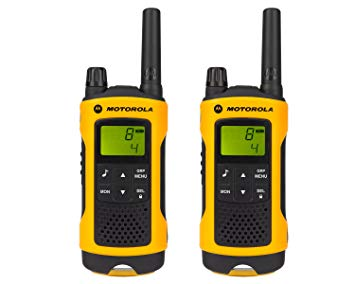
\includegraphics[width=0.5\textwidth]{walkies.jpg}
\caption{Pareja de \textit{walkies} \ac{PMR}. \protect\footnotemark}
\label{fig:walkies}
\end{center}
\end{figure}
\footnotetext{Imagen original extraída de \url{https://images-na.ssl-images-amazon.com/images/I/71Dz7lkZzVL._SX355_.jpg}}

El Canal 7-7 \ac{PMR}\footnote{\url{http://www.canal77pmr.com/}} consiste en una estrategia que busca que todos los grupos de montaña y los montañistas individuales usen el Canal 7 y el Subtono 7 (frecuencia de canal de 446.08125MHz y frecuencia de subtono de 85.4Hz) como medio de comunicación. Esta estrategia surgió al buscar a un deportista perdido en la montaña, ya que era necesario que todas las personas que participaban en la búsqueda se comunicasen en un mismo canal y subtono.

\begin{figure}[!h]
\begin{center}
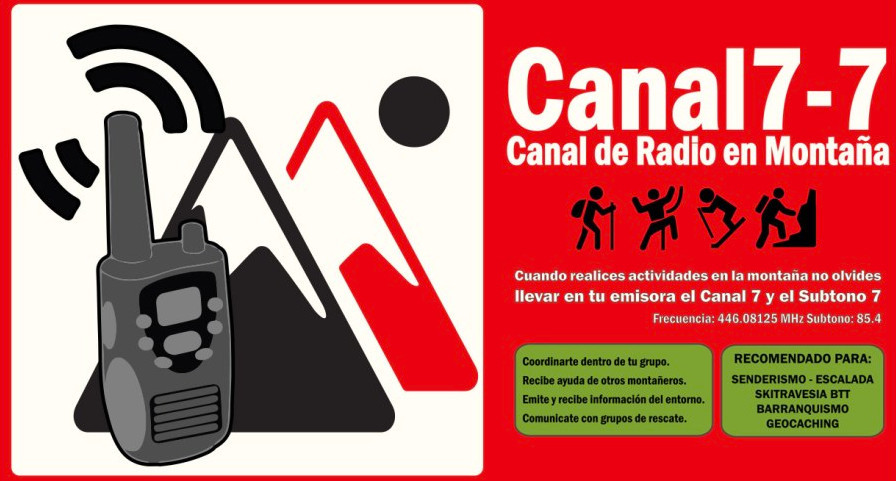
\includegraphics[width=0.5\textwidth]{canal77.jpg}
\caption{Anuncio para el uso del Canal 7-7 en la montaña. \protect\footnotemark}
\label{fig:canal77}
\end{center}
\end{figure}
\footnotetext{Imagen original extraída de \url{https://pmrjaen.files.wordpress.com/2018/02/canal77.jpg?w=900}}

\section{Estructura del documento}

El presente \ac{TFG} se compone de los siguientes capítulos:

\begin{definitionlist}
\item \textbf{Capítulo \ref{chap:intro}. \nameref{chap:intro}} \\
Se trata del capítulo actual. En él se plantea la problemática existente que se pretende resolver con este \ac{TFG}.
\item \textbf{Capítulo \ref{chap:objetivos}. \nameref{chap:objetivos}} \\
En este capítulo se presentan los objetivos a alcanzar que se deben satisfacer en el desarrollo del \ac{TFG}, para alcanzar el éxito en el mismo.
\item \textbf{Capítulo \ref{chap:metodo}. \nameref{chap:metodo}} \\
En este capítulo se muestra la metodología de desarrollo que se ha llevado a cabo durante el presente proyecto, además de las distintas herramientas usadas para el mismo. Se presentarán también las distintas fases para la elaboración de este \ac{TFG}.
\item \textbf{Capítulo \ref{chap:resultados}. \nameref{chap:resultados}} \\
Este capítulo muestra los resultados obtenidos, fruto de las pruebas realizadas con el prototipo desarrollado.
\item \textbf{Capítulo \ref{chap:conclusiones}. \nameref{chap:conclusiones}} \\
\end{definitionlist}

% Local Variables:
%  coding: utf-8
%  mode: latex
%  mode: flyspell
%  ispell-local-dictionary: "castellano8"
% End:
